
\documentclass{beamer}
\usetheme{umbc1}

%%% Packages
% First four - AMS (american mathematical society). General math goodness. I use the align* enviorment in particular
% multirow, multicol allow for certain kinds of tables
% enumerate lets you determine the style of the counter for the enumerate enviorment
% graphicx lets you include pictures
% listings lets you stick in blocks of code
% placeins defines "\FloatBarrier", which stops tables from moving around
\usepackage{amsmath, amscd, amssymb, amsthm, multirow, multicol, enumerate, graphicx, listings, placeins} 
\newcommand{\Z}{\mathbb{Z}}
\newcommand{\R}{\mathbb{R}}
\newcommand{\Q}{\mathbb{Q}}
\newcommand{\C}{\mathbb{C}}
\newcommand{\N}{\mathbb{N}}
\newcommand{\V}{\mathbb{V}}
\newcommand{\U}{\mathcal{U}}
\newcommand{\del}{\partial}
\newcommand{\real}{\textrm{Re }}
\newcommand{\imag}{\textrm{Im }}
\newcommand{\pd}[2]{\frac{\partial #1}{\partial #2}}
\newcommand{\deriv}[2]{\frac{d #1}{d #2}}
\newcommand{\sumk}{\sum_{k=1}^\infty}
\newcommand{\sumj}{\sum_{j=1}^\infty}
\newcommand{\sumn}{\sum_{n=0}^\infty}
\newcommand{\summ}[2]{\sum_{k=#1}^{#2}}
\newcommand{\sig}[1]{\sum_{#1 =1}^\infty}
\newcommand{\un}[1]{\bigcup_{#1 =1}^\infty}
\newcommand{\inter}[1]{\bigcap_{#1 =1}^\infty}
\newcommand{\ip}[2]{\langle #1, #2 \rangle}
\newcommand{\ipxu}{\langle x,u_j \rangle}
\newcommand{\uj}{\{u_j\}_{j=1}^\infty}
\newcommand{\B}{\mathcal{B}}

\newcommand{\p}{\mathrm{P}}
\newcommand{\E}{\mathrm{E}}
\newcommand{\var}{\mathrm{Var}}
\newcommand{\cov}{\mathrm{Cov}}
\newcommand{\ST}{mbox{ s.t. }}

\newcommand{\st}{ \; \big | \:}

\newcommand{\deuc}{d_{\mathrm euc}}
\newcommand{\dtaxi}{d_{\mathrm taxi}}
\newcommand{\ddisc}{d_{\mathrm disc}}

\newcommand{\hwhead}[1]{#1 \hfill Aaron Maurer \vspace{2mm} \hrule \vspace{2mm}}
\newcommand{\diag}[1]{\mathrm{diag}\{#1\}}
\DeclareMathOperator*{\argmin}{arg\min}

\title{Using Probabilistic Knockoffs of Binary Variables to Control the False Discovery Rate}
\author{Aaron Maurer \\ Advisor: Rina Foygel Barber}
\date{July 29th, 2015}

\begin{document}
%%%%%%%%%%%%%%%%%%%%%%%%%%%%%%%%%%%%%%%%%%%%%%%%%%%%%%%%%%%%%%%%%%%%%%%%%%%%%%%%%%%%%%%%%%%%%%%%%%%%%%%%%%%%%%%%%%%%%%%%%%%%%%%%%%%%%
\begin{frame}[plain]
    \titlepage
\end{frame}

\begin{frame}{Overview}
    \begin{enumerate} 
        \item Original Knockoffs: What They Do and Where They Fail
        \item Making Knockoffs Work With GLMs
        \item Random Binary Knockoffs: The Theory
        \item Random Binary Knockoffs: Performance
        \item Where to next?
    \end{enumerate}
\end{frame}

\begin{frame}{Variable Selection in Linear Regression}
    Assume
     \[\mathbf{y} = X\beta + \mathbf{z}\]
    where $\mathbf{y}\in\R^n$, $X \in \R^{n\times p}$, $\beta\in\R^p$, and $\mathbf z$ is Gaussian noise. Also, assume sparsity:
    \[\beta_i = 0 \quad \forall i\not\in S\]
    How do we choose a model $\hat S$?
\end{frame}

\begin{frame}{False Discovery Rate}
    A common goal for a method that generates $\hat S$ is to control the false discovery rate
    \[ \textrm{FDR} = \E\left[\frac{\vert{\{j: \beta_j=0 \; \& \; j\in\hat S\}}\vert}{\max\{\vert{\hat S}\vert,1\}} \right] \]
    In other words, control proportion of elements in $\hat S$ which aren't in $S$. \par
    \vspace{1cm}
    FDR is controlled at level $q$ if $q\geq$FDR irrespective of true $\beta$.
    
\end{frame}

\begin{frame}{Knockoff Features}
    Knockoff variables can be used to control FDR in linear regression. 
    \begin{itemize}
        \item The idea is to create a forgery of each variable; if the forgeries seem about as good predictors as the originals, the originals are lousy predictors.
        \item For each variable $X_i$, create a knockoff feature $\tilde X_i$ such that, where $X^TX=G$, $\diag{X^T X} - s$ is small and 
            \[ \tilde X^T \tilde X = G \quad \& \quad X^T \tilde X = G - \diag{\mathbf s} \]
        \item $\tilde X_i$ and $X_i$ will have same correlation with other variables, but only low correlation with each other.
        \item For $\tilde X$ to exist, it must be the case that
            \[ G_L =[X\; \tilde X]^T[X\; \tilde X] = \left[ \begin{array}{cc} G & G - \diag{\mathbf s} \\ G - \diag{\mathbf s} & G \end{array}\right] \succeq 0 \]
        \item Given $\mathbf s$, $\tilde X$ can be generated via a rotation of $X$.
    \end{itemize}
\end{frame}

\begin{frame}{Knockoff Filter}
    These knockoffs can be used in the knockoff filter method. 
    \begin{itemize}
        \item Fit full path of LASSO regression on $[\,X\,\tilde X\,]:=X_L$.
    \[ \beta(\lambda) = \argmin_\mathbf b \left\{\frac{1}{2}\|\mathbf y - X_L\mathbf b\|^2_2 + \lambda\|b\|_1 \right\}\]
        \item $Z_i$, $\tilde Z_i$ are the largest $\lambda$ such that $X_i$, $\tilde X_i$ have nonzero coefficient.
        \item $W_i= Z_i$ if $Z_i>\tilde Z_i$, otherwise $W_i = -\tilde Z_i$.
        \item Since $G_L$ \& $[\, X \, \tilde X\,]^T\mathbf y$ are sufficient statistics for $\beta(\lambda)$, $W_i$ symmetrically distributed around $0$ when $X_i$ null predictor.
        \item Thus, FDR controlled when $\hat S = \{i:W_i\geq T\}$ for 
            \[ T = \min\left\{ t>0 \;: \; \frac{\vert\{j:W_j\leq -t\}\vert}{\max\{\vert\{j:W_j\geq t\}\vert,1\}}\leq q \right\} \]
    \end{itemize}
\end{frame}

\begin{frame}{Variable Selection in GLMs}
    Knockoffs work great for linear regression, but what about GLMs? \\
    \vspace{1cm}
    Now, assume, for some link function $g$ and $y_1,\ldots,y_n$ from a exponential family distribution,
     \[\E(\mathbf{y}) = g(X\beta)\]
    where $X \in \R^{n\times p}$ and $\beta\in\R^p$. Also, assume sparsity:
    \[\beta_i = 0 \quad \forall i\not\in S\]
    How do we choose a model $\hat S$?
\end{frame}

\begin{frame}{Where Knockoff Filter Fails}
    Knockoff filter doesn't work for other GLMs. \\
    \begin{center}
        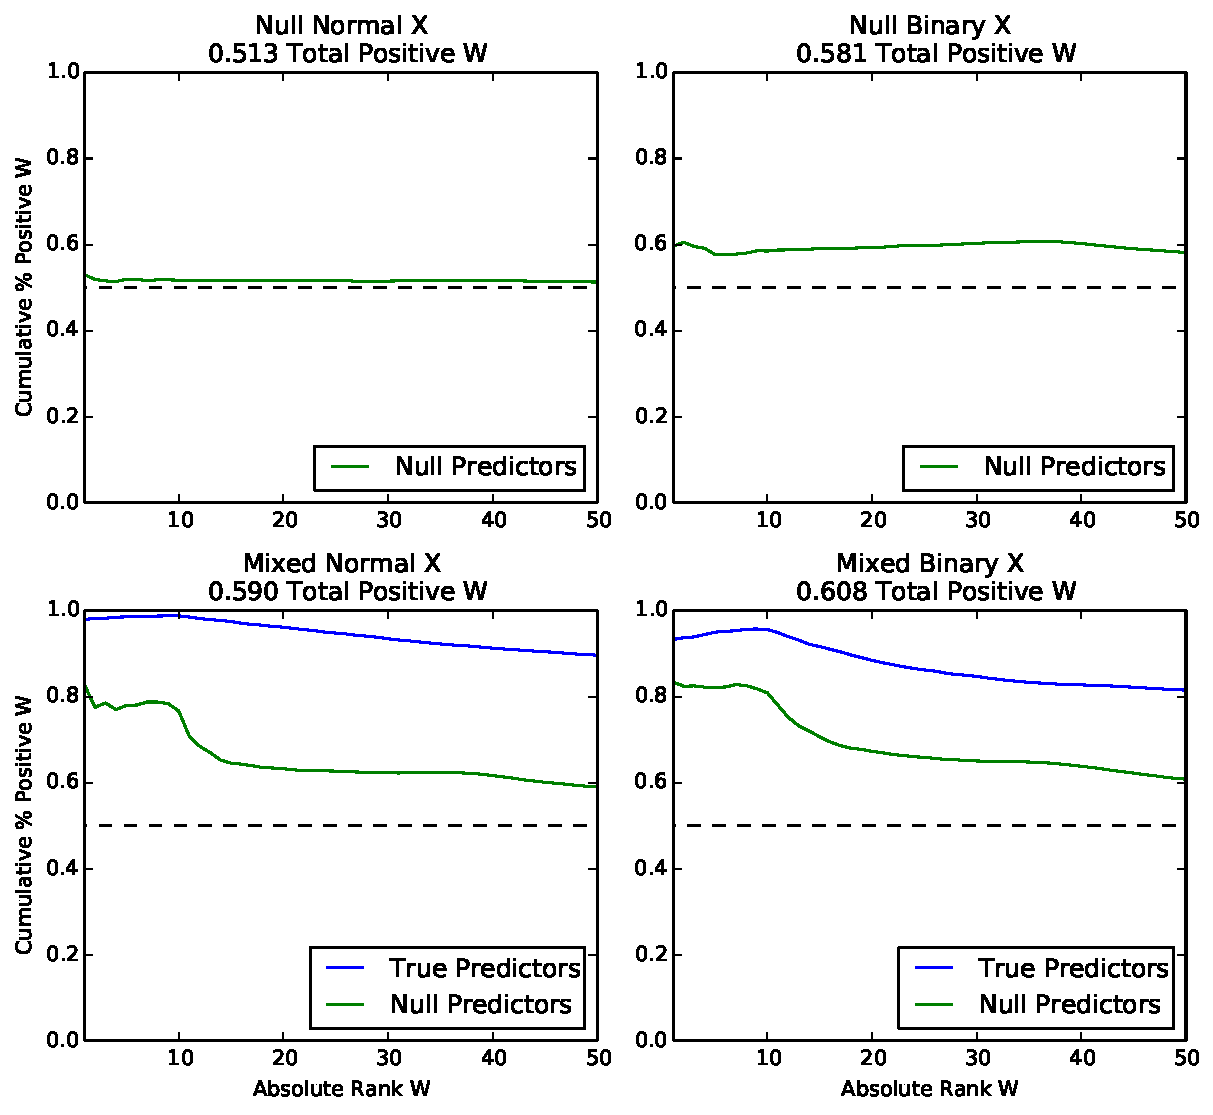
\includegraphics[width=8cm]{images/entryrate_original_logit}
    \end{center}
\end{frame}

\begin{frame}{Can Knockoffs Be Fixed for GLMs?}
    \begin{itemize}
        \item Other GLMs don't have the same sufficient statistics as linear regression.
        \item Original Knockoffs don't remotely have same distribution as $X$, so ``look'' different than real variables.
        \item Knockoffs will likely work better if they have the same marginal distribution as originals. 
        \item For $X_i$ with arbitrary distribution, unclear how this might be accomplished.
    \end{itemize}
\end{frame}

\begin{frame}{Random Binary Notation}
    \begin{itemize}
        \item Binary data is common in data analysis and a much more manageable family of distributions for $X$.
        \item We can think of observations in $X$ as observations of random binary vector $\mathbf x\in\{0,1\}^p$.
        \item The full family for $\mathbf x$ is multinomial on $2^p$ outcomes.
        \item Can summarize with the first two moments: 
            \[ \E(\mathbf{x}\mathbf{x}^T) = M \in [0,1]^{p\times p} \quad \& \quad \diag{M} = \E(\mathbf x) = \mathbf{m} \in [0,1]^p  \]
        \item For arbitrary $M$ to correspond to a random binary vector, must be case that $ M-\mathbf{m}\mathbf{m}^T = \Sigma \succeq0$
            \[\max\{0,m_i+m_j -1\} \leq M_{ij} \leq \min\{m_i,m_j\} \]

    \end{itemize}
\end{frame}

\begin{frame}{Random Binary Knockoffs}
    \begin{itemize}
        \item Integer programing is NP-hard, making finding $\tilde X\in\{0,1\}^{n\times p}$ to fit correlations optimally difficult. 
        \item Instead, introduce a relaxed problem where $\tilde X\st X$ is drawn randomly such that, where $\Sigma=\cov(\mathbf x)$
            \[ \cov(\mathbf{\tilde x}, \mathbf x) = \Sigma - \diag{\mathbf s} \quad \& \quad \cov(\mathbf{\tilde x}) = \Sigma \]
        \item For this to correspond to a random binary vector, must be the case
            \[ \Sigma_L =\cov([\,\mathbf x\,\mathbf{\tilde x}\,]) = \left[ \begin{array}{cc} \Sigma & \Sigma - \diag{\mathbf s} \\ \Sigma - \diag{\mathbf s} & \Sigma \end{array}\right] \succeq 0 \]
        \item Almost same correlation condition as before, but only holds in expectation.
        \item Switch from Gramian matrix to correlation matrix makes moment condition less likely to be violated. 
    \end{itemize}
\end{frame}

\begin{frame}{Quadratic Programing}
    \begin{itemize} 
        \item Simplest approach to is to draw the entries of $\tilde X$ independently based on probabilities $P\in[0,1]^{n\times p}$.
        \item $P$ should satisfy 
            \begin{center}
                \begin{tabular}{r l}
                    minimize     & $\|X^TP-(M-\diag{s})\|_{fro}^2 + \sum_{i\neq j}(P_i^T P_j - M_{ij})^2 $\\
                    subject to   & $ \mathbf 1^T P = \mathbf m $ \\
                                 & $0 \leq P \leq 1$
                \end{tabular} 
            \end{center}
        \item Can be formulated as a quadratic program with slack variables
            \begin{center}
                \begin{tabular}{r l}
                    minimize     & $\|W\|_{fro}^2 + \|V\|_{fro}^2 $ \\
                    subject to   & $ -W \leq X^TP-(M-\diag{s})\leq W $ \\
                                 & $ -V_{ij} \leq P_i^T P_j - M_{ij} \leq V_{ij} \quad \forall i\neq j$ \\
                                 & $ \mathbf 1^T P = \mathbf m $ \\
                                 & $0 \leq P \leq 1$
                \end{tabular} 
            \end{center}
        \item Huge optimization problem, likely computationally difficult.
    \end{itemize}
\end{frame}

\begin{frame}{Ising Model}
    \begin{itemize}
        \item Alternatively, find a random binary vector variable $\mathbf{x}_L$ that has cross-moments $M_L$ corresponding to $\Sigma_L$.
        \item The Ising model can match any proper $M_L$. If $A$ is a lower triangular matrix and $L$ the logistic link function
            \[ \p(\mathbf x=\mathbf \gamma) \propto L(\mathbf{\gamma}^T A\mathbf \gamma)\]
        \item The Ising model binary analog of normal distribution; maximum entropy for given covariance matrix.
        \item Very easy to draw successive entries
            \[ \p(x_{i}=1\st x_{1},...,x_{i-1}) = L\left(A_{ii}+\sum_{k=1}^{i-1}A_{ik}x_i\right) \]
        \item Once fit, can draw $\mathbf{\tilde x}\st \mathbf x$ easily.

    \end{itemize}
\end{frame}

\begin{frame}{Fitting Ising Model}
    \begin{itemize}
        \item If we were just trying to fit $A$ to $X$, we could do so via successive logistic regression to fit row $\mathbf a_i$.
        \item Instead, simulate $\mathbf m_i = f(\mathbf a_i)$ and fit via Newton-Raphson. 
        \item Draw $K$ samples $\mathbf x_{-i}^{(k)}\sim \mathbf x_{-i}$. Then
            \[f\left(\mathbf a_i\right) \approx \frac{1}{K}\sum_{k=1}^K L\left(\mathbf{a}_i^T\left[\begin{array}{c} \mathbf x_{-i}^{(k)} \\ 1 \end{array}\right]\right)\left[\begin{array}{c} \mathbf x_{-i}^{(k)} \\ 1 \end{array}\right] \]
            \[J\left( \mathbf a_i\right) \approx \frac{1}{K}\sum_{k=1}^K L'\left(\mathbf{a}_i^T\left[\begin{array}{c} \mathbf x_{-i}^{(k)} \\ 1 \end{array}\right]\right)\left[\begin{array}{c} \mathbf x_{-i}^{(k)} \\ 1 \end{array}\right]\left[\begin{array}{cc} \mathbf [x_{-i}^{(k)}]^T & 1 \end{array}\right] \]
        \item Make successive updates
            \[\mathbf a_i^{(k+1)} = \mathbf a_i^{(k)} - \left[J\left(\mathbf a_i^{(k)}\right) \right]^{-1}\left[f\left(\mathbf a_i^{(k)}\right)-\mathbf m_i\right] \]
    \end{itemize}
\end{frame}

\begin{frame}{Computational Issues}
    \begin{itemize}
        \item $K$ must be very large for big $p$ and high correlation.
        \item This makes $J\left( \mathbf a_i\right)$ and even $f\left(\mathbf a_i\right)$ very expensive to calculate.
        \item This makes quasi-Newtonian methods, where $J\left( \mathbf a_i\right)$ is approximated, appealing.
        \item In particular, Anderson Mixing, where $f$ approximated with secant hyperplane through $\mathbf a_i^{k},\ldots,\mathbf a_i^{(k-h+1)}$ works well
        \item When $K$ too small, can instead solve relaxed problem
    \[\mathbf m_i^*(\tau) = (1-\tau)\mathbf m_i + \tau \left[ \begin{array}{cccc} 0 & \ldots & 0 & M_{ii} \end{array} \right]^T \]
        \item $n$ doesn't matter, but this method is also fairly impractical for large $p$.
    \end{itemize}
\end{frame}

\begin{frame}{Random Binary Knockoffs in Linear Regression}
    Random binary Knockoffs only provide approximate FDR control for linear regression. 
    \begin{center}
        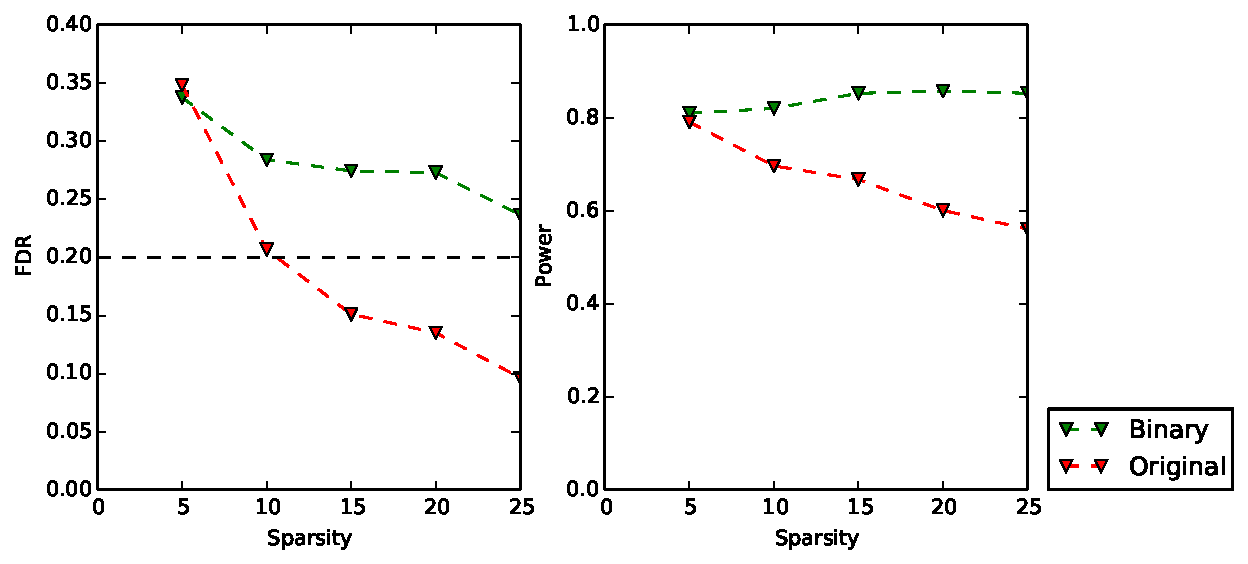
\includegraphics[width=11cm]{images/lasso_FDR_power_50}
    \end{center}
    They select too many variables, causing higher power at the expense of FDR control.
\end{frame}

\begin{frame}{Distortion from $M_L$}
    Since $\tilde X$ is randomly generated, $\frac{1}{n}X_L^TX_L$ deviates from $M_L$.
    \begin{center}
        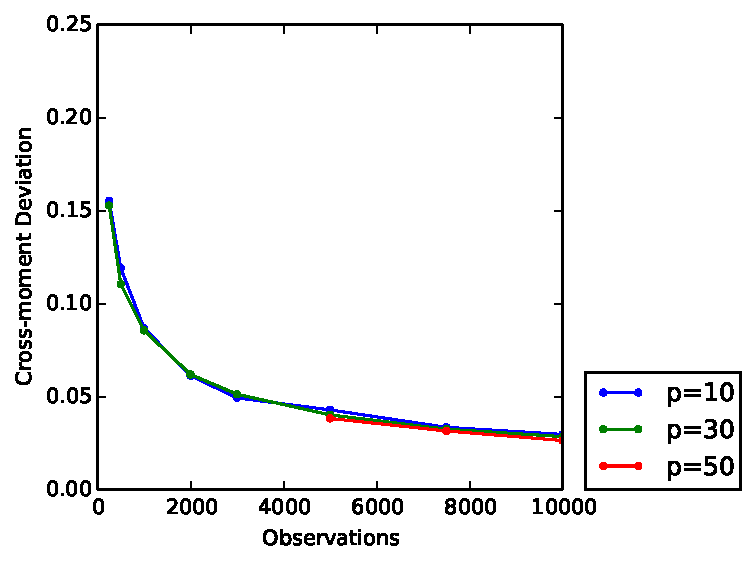
\includegraphics[width=8cm]{images/sigma_fit}
    \end{center}
    As $n$ increases, this effect diminishes. 
\end{frame}

\begin{frame}{Random Binary Knockoffs in Logistic Regression}
    Random Binary Knockoffs perform much better than original knockoffs in logistic regression.
    \begin{center}
        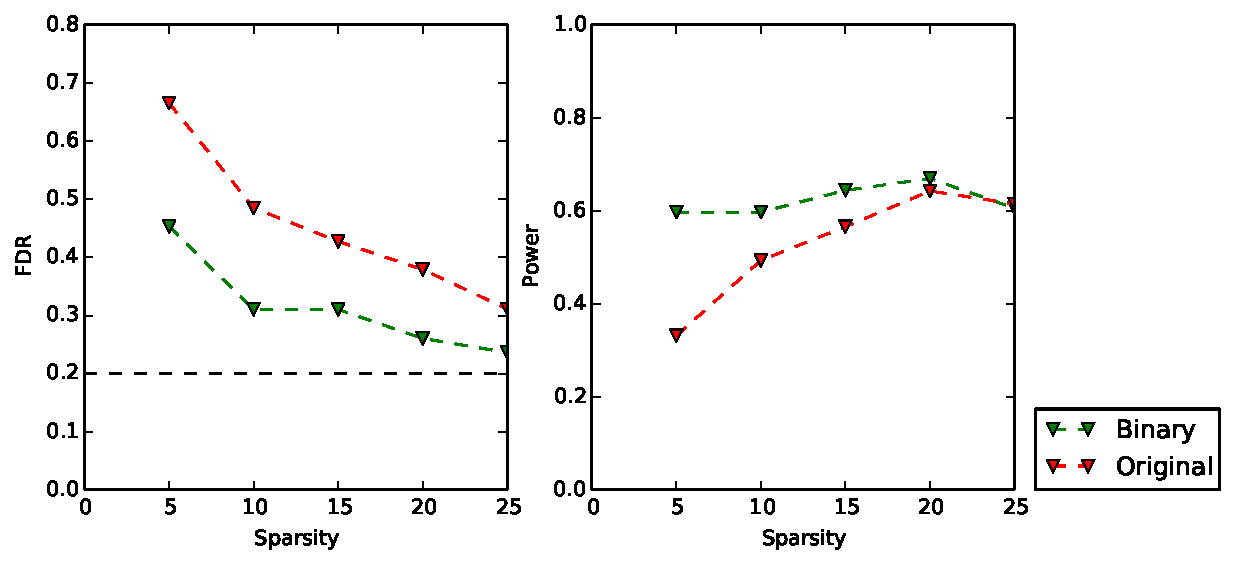
\includegraphics[width=11cm]{images/logit_FDR_power_50}
    \end{center}
    They have lower FDR and higher power.
\end{frame}

\begin{frame}{Discussion}
    \begin{itemize}
        \item Random Binary Knockoffs seem to offer promise as a useful technique, but have outstanding issues.
        \item Seem to offer a method to extend Knockoffs for one type of variable to GLMs.
        \item Computational complexity prohibitive; simpler method, perhaps by good approximation of $P$, would be helpful.
        \item Random distortion from desired cross-moments might be compensated for by ensemble method based on multiple $\tilde X$.
        \item Might build higher order interactions into Ising model to allow for nasty data.
    \end{itemize}
\end{frame}

\end{document}
